\documentclass{article}

% enable these lines below while using overleaf, disable for texmaker/latex workshop
%\usepackage[utf8]{inputenc}
%\usepackage{stmaryrd}
%\usepackage{algorithm,algpseudocode} 
%\usepackage{galois}

\usepackage{xspace}
\usepackage{amsmath}
\usepackage{afterpage}
\usepackage{graphicx,lipsum}   
\usepackage{figlatex,wrapfig}
\usepackage[dvipsnames]{xcolor}
\usepackage{listings,amssymb,mathtools}
\usepackage{mathrsfs}
\usepackage{array,multirow}
\usepackage{pifont}
\usepackage{caption}
\usepackage{geometry}
\usepackage{textcomp}
\usepackage{algorithm}
\usepackage[noend]{algpseudocode}

\usepackage{tikz}
\usepackage[shortlabels]{enumitem}

% for colours
\usepackage{xspace}
\usepackage[colorlinks]{hyperref}
\hypersetup{
	colorlinks = true,
	citecolor = {violet},
	linkcolor = {blue},
	urlcolor  = {blue}
}

% for arrow diagrams
\usepackage{amsmath}
\usepackage{amssymb}
\usepackage{smartdiagram}
\usepackage{tikz}
\usetikzlibrary{arrows,positioning}

\usepackage[parfill]{parskip}

% for bib handline
\usepackage[numbers]{natbib}
\usepackage{url}

\definecolor{brown}{rgb}{0.59, 0.29, 0.0}
\definecolor{green}{rgb}{0.0, 0.5, 0.0}
\definecolor{orange}{rgb}{1.0, 0.62, 0.0}
\definecolor{purple}{rgb}{0.5, 0.0, 0.5}
\definecolor{red}{rgb}{1.0, 0.0, 0.0}
\definecolor{blue}{rgb}{0.0, 0.0, 1.0}

\newcommand{\mosc}{\texttt{seq\_cst}\xspace}
\newcommand{\moacqrel}{\texttt{acq\_rel}\xspace}
\newcommand{\morel}{\texttt{release}\xspace}
\newcommand{\moacq}{\texttt{acquire}\xspace}
\newcommand{\mocon}{\texttt{consume}\xspace}
\newcommand{\morlx}{\texttt{relaxed}\xspace}

\newcommand{\seqb}[2]{{#1} {\color{brown}$\rightarrow^{sb}$} \color{black}{#2} }
\newcommand{\sw}[2]{{#1} {\color{purple}$\rightarrow^{sw}$} \color{black}{#2} }
\newcommand{\hb}[2]{{#1} {\color{orange}$\rightarrow^{hb}$} \color{black}{#2}}
\newcommand{\rf}[2]{{#1} {\color{blue}$\rightarrow^{rf}$} {#2} }
\newcommand{\too}[2]{{#1} {\color{green}$\rightarrow^{to}$} {#2} }
\newcommand{\mo}[2]{{#1} {\color{red}$\rightarrow^{mo}$} {#2} }
\newcommand{\setSB}{{\color{brown}\tt{sb}}\xspace}
\newcommand{\setSW}{{\color{purple}\tt{sw}}\xspace}
\newcommand{\setRF}{{\color{blue}\tt{rf}}\xspace}
\newcommand{\setHB}{{\color{orange}\tt{hb}}\xspace}
\newcommand{\setTO}{{\color{green}\tt{to}}\xspace}
\newcommand{\setMO}{{\color{red}\tt{mo}}\xspace}

\newcommand{\var}[1]{\color{OliveGreen}\texttt{#1}\color{black}}
\newcommand{\fun}[2]{\color{Sepia}\texttt{#1(\color{Gray}\textit{#2}\color{Sepia})}\color{black}}
\newcommand{\class}[1]{\color{DarkOrchid}\texttt{#1}\color{black}}

\newcommand{\ishComment}[1]{\textit{\color{red}\tiny{#1}}}
\newcommand{\divComment}[1]{\textit{\color{green}{#1}}}

\title{fence-synthesis-paper}
\date{}

\begin{document}

\maketitle
\textit{\textbf{Abstract-}}

\section{Introduction} \label{sec:intro}
% ------------ INTRO PARAS ------------------
\par
A programmer working with relaxed memory constraints would want all the advantages of the relaxed model - such as speed and concurrency. However, using relaxed memory constraints comes with its own issues. In relaxed memory models, memory operations such as \textit{reads} and \textit{writes} can be reordered in order to achieve these properties. These instruction reorderings can cause certain variables to have different values in different execution runs of the same program, hence resulting in behaviour which is unexpected or surprising. These include not behaving according to sequentially consistent standards, or outputting unexpected values of variables.

\par
In this project, we suggest an approach to prevent certain unexpected behaviour, such as unexpected outputs due to concurrent instruction re-orderings in the C11 relaxed model.

\par
To tackle this, the programmer may add \textit{"assert"} statements in the source code, which will check that certain properties remain unchanged in each run of the program, such as the value of a variable in a certain thread. Each program will have several possibilities of runs where instructions will be executed in different orders. In some of these runs, there might be cases where the assertion does not hold and it gets violated. In the case that the \textit{assert} statement gets violated, the program execution will stop. The object of this project is to insert a minimum number of \textbf{C11 fences} in the source code of the program at the right places so that these assertions are satisfied and do not get violated.

% -------------------- MOTIVATION E.G. ------------------------
\subsection{Motivation Example}

% -------------------- FIG 1: BASIC ------------------------
\begin{figure}[!htb]
\begin{center}
\texttt{
init y := 0, x := 0;\\
	\begin{tabular}{c l || c l}
		(1) & y := 1 & (5) & x := 1\\
		(2) & if x == 0 & (6) & if y == 0\\
		(3) & \qquad c := 1 & (7) & \qquad c := 0\\
		(4) & \qquad t = c \color{olive}//1 & (8) & \qquad t = c \color{olive}//0
	\end{tabular}
}
	\caption{Simple two-thread dekker program}\label{fig:dekker1}
\end{center}
\end{figure}
\ishComment{to use R, W here as well? to show atomic operations? to use brackets for if?}

\par
In a sequentially consistent model, the multi-threaded program in Fig \ref{fig:dekker1} would execute the instructions in a sequentially consistent order. The final values read by variable \textit{t} would be 1 and 0 for each thread respectively. Therefore it can be said that the ``output'' would always be ``10''. However, in the case of a relaxed model, such as in a C11/C++11 program when all the instructions are relaxed, reading outputs of ``00'', ``01'', ``11'' may even be possible, thereby violating the rules of sequential consistency. Such an output may or may not be unexpected for the programmer, depending upon their requirements.

\par
For this reason, the programmer needs to provide their requirements about what values are expected at which locations by specifying a local safety property.

% --------------- FIG 2.2 basic + assert -------------
\begin{figure}[!htb]
\begin{center}
\texttt{
init y := 0, x := 0;\\
	\begin{tabular}{c l || c l}
		(1) & W$\mathtt{_{rel}}$y(1) & (5) & W$\mathtt{_{rel}}$x(1)\\
		(2) & if R$\mathtt{_{rel}x}$ == 0 & (6) & if R$\mathtt{_{rel}y}$ == 0\\
		(3) & \qquad W$\mathtt{_{rel}}$c(1) & (7) & \qquad W$\mathtt{_{rel}}$c(0)\\
		(4) & \qquad assert($\mathtt{R_{rel}c}$ == 1) & (8) & \qquad assert($\mathtt{R_{rel}c}$ == 0)
	\end{tabular}
}
	\caption{Simple two-thread dekker program in C11 syntax with assertions}\label{fig:dekker2}
\end{center}
\end{figure}

\par
Such a specification may be made in the form of assertions such as those described in Fig \ref{fig:dekker2} This ``assert'' statement checks that the expression provided to it holds at that point in the program. At the end of the threads, this safety property might not be satisfied. In this case, the program stops or exits, giving an error output. The objective of the tool to be created is to prevent the program from exhibiting behaviour which is unexpected for the programmer, hence preventing the error output as well as ensuring the provided specifications. For the purposes of this paper, we require the safety property to be specified as assertions in the program.

\section{Related Work} \label{sec:related}
The literature in the  fence synthesis is dominated by 
techniques targeting the x86-TSO and sparc PSO memory models
such as \cite{abdulla2012counter}\cite{alglave2010fences}
\cite{alglave2014don}\cite{linden2011verification}
\cite{abdulla2012automatic}\cite{abdulla2015best}
\cite{bender2015declarative} for x86-TSO,
\cite{abdulla2015precise}\cite{linden2013verification} 
for sparc PSO and \cite{liu2012dynamic}
\cite{meshman2014synthesis}\cite{abdulla2013memorax}
\cite{joshi2015property}\cite{kuperstein2012automatic}
for both TSO and PSO.
%
The technique \cite{bender2015declarative} additionally
provides fence synthesis for ARMv7 memory model and 
\cite{kuperstein2012automatic} additionally provides
fence synthesis for RMO memory model.
%
Apart from the techniques for TSO and PSO, a few 
fence synthesis techniques have been proposed for Power
memory model \cite{alglave2010fences}\cite{abdulla2015precise}
\cite{fang2003automatic}; \cite{fang2003automatic} also 
provides support for IA-32 memory model.

Some of the earlier works in the area \cite{alglave2010fences}
\cite{abdulla2015precise}\cite{fang2003automatic} 
perform fence synthesis to reduce a weak memory behaviors of an 
input program to those permitted under Sequential Consistency (SC)
or its variant \cite{abdulla2015best}.
%
Most techniques \cite{

\section{Background/Preliminaries} \label{sec:prelim}
% -------------------- C11 MODEL ------------------------
\subsection{The C11 Model}
\par
Since the C/C++11 memory model is a relaxed model, load/store operations can be re-ordered before they are stored into the memory. In multi-threaded programs due to re-orderings between loads and stores, and other factors such as different methods used by different hardware for cache coherency, threads may end up seeing loads and stores by other threads in an order different than the one intended. One way of controlling this is through specifying the memory order for each operation in the program.

\begin{figure}
	\begin{center}
		\begin{tabular}{|c|}
		\hline
		non-atomic $<$ relaxed $<$ release = acquire $<$ sequential consistency\\
		\hline
		\end{tabular}
	\caption{Memory orders in increasing order of strength}\label{fig:mo_strength}
	\end{center}
\end{figure}

As discussed previously, this feature can cause behaviour which is unexpected by the programmer. Two memory consistency primitives introduced into the C/C++11 model can be exploited by us in this scenario - \textit{atomic operations} and \textit{memory fences}. 

% ------------- ATOMIC OPS ----------------
\subsubsection{Atomic Operations}
Examples of atomic operations in the C/C++11 memory order are atomic loads, atomic stores, atomic read-modify-writes. These operations are carried out on atomic objects/variables.

\ishComment{insert examples of atomic ops like a.load(mo\_rel) etc}

The approach described in this project makes use of these atomic operations within the input program.

% --------------- FENCES ----------------
\subsubsection{C11 Fences}
\par
A fence in the C11 model is also an atomic instruction which can be inserted between other instructions. These fences prevent memory operations to be ordered or re-ordered past the fence and they also permit the operations to be ordered in-between threads. 

\par
A fence can have memory order SC, release, acquire. Specifically, a release fence prevents previous load/store operations from being re-ordered and moved after the fence and an acquire fence prevents load/store operations after the fence to be re-ordered and moved before the fence. On the other hand, an SC fence prevents both such behaviours. This project focuses only on SC fences and inserting them into the program in order to methodically stop instructions from re-ordering and preventing the unexpected behaviour.
\ishComment{behaviour spelling}

% ---------------- TYPES OF RELATIONS -----------
\subsection{Basic relations}
\par
In a program execution, there can be certain relations formed between instructions. Each type of relation has rules or preconditions which dictate the type of relation between any two instructions.

\par
Three basic relations which are useful in calculating many other relations are the \textit{sequenced-before}, \textit{synchronizes-with} and \textit{read-from} relations. In basic terms, any instruction in a thread is said to be sequenced before all instructions that are evaluated after it in the same thread. In order to concurrently access shared variables in a synchronized manner to avoid data races, the \textit{synchronizes-with} relation is used among instructions from different threads. Finally, a read instruction is said to be \textit{reading-from} the value of a write instruction.

These relations form the basis for all other relations which are required in the methodology of this paper. These relations are \textit{happens-before}, \textit{modification order} and \textit{total order}.

% ---------------- NOTATIONS -----------
\subsection{Notation}
\begin{itemize}
	\item F$_{mo}$ \qquad fence with memory order mo
	\item Rx \qquad read/load or rmw atomic operation on variable x
	\item Wx(a) \qquad write/store or rmw atomic operation storing value a in variable x
	\item R$_{mo}$ \qquad memory order mo specified for read operation
	\item W$_{mo}$ \qquad memory order mo specified for write operation
	\item $_{\geq rel}$ \qquad memory orders greater than or equal to release according to Fig. \ref{fig:mo_strength}
	\item := \qquad assignment operator
	\item == \qquad comparison operator
	\item \color{olive}//a \color{black} \qquad the value expected to be read in that line is a
	\item rmw
	\item sb, sw, rf, hb, mo, to \qquad \too{a}{b} etc 
	\item seq\_cst, rel, acq, rel\_acq, rlx
	\item thread A create \qquad spawn a thread A from the current thread
	\item thread A start \qquad the first/starting instruction of a thread A
	\item thread A finish \qquad the last/ending instruction of a thread A
	\item thread A join \qquad when a thread A joins back into the spawning thread
	\item || separation of threads
	\item buggy traces / buggy executions
\end{itemize}

\section{Proposed Solution/Our Approach}\label{sec:approach}
Given a buggy input program $P$, \ourtechnique attempts to 
stop the buggy traces or counter examples (traces with 
assert statement violations) of $P$ by inserting \cc fences.
%
To do so the technique must accomplish three objectives
(O1) determine whether the buggy trace can be stopped by 
synthesizing \cc fences,
(O2) determine the placement of optimal number of synthesized 
fences (\ie the least number of program locations where fences 
must be synthesized that is sufficient to stop the trace), 
and
(O3) determine the optimal memory order of the synthesized 
fences (\ie the weakest memory order of synthesized fences 
that is sufficient to stop the trace).
%
We present the \ourtechnique-algorithm (Algorithm
\ref{alg:main algo}) that realizes the three objectives.
The algorithm takes a \cc program as input
and determines the optimal fence placement that can stop
the buggy traces of the input program or determines that
the program cannot be made bug-free with \cc fences.

\begin{algorithm}[h]
	\caption{Fence Synthesis}
	\label{alg:main algo}
	\DontPrintSemicolon
	\SetAlgoLined
	
	\SetKwFunction{Fmain}{\ourtechnique}
	\SetKwFunction{Fceg}{generateCounterExamples}
	\SetKwFunction{FcandidateF}{candidateFences}
	\SetKwFunction{Frel}{computeRelations}
	\SetKwFunction{Fwk}{weakFensying}
	\SetKwFunction{Fst}{strongFensying}
	\SetKwFunction{Fmin}{minModel}
	
	\SetKwData{satquery}{$\Phi$}
	\SetKwData{ce}{CE}
	\SetKwData{wk}{weakCycles}
	\SetKwData{st}{strongCycles}
	
	\SetKwProg{Fn}{Function}{:}{}
	
	\Fn{\Fmain{input program $P$}}{		
		\satquery $:=$ $\top$\;
		\ce $:=$ \Fceg{$P$}\;
		\ForAll(\tcc*[f]{$\tau = \langle \events_\tau, \setHB, \setMO, \setRF \rangle$}) {$\tau \in$ \ce}{
			$\events_{\imm{\tau}}$ $:=$ $\events_\tau$ $\union$ \FcandidateF{$\tau$}\;
			$(\hb{\imm{\tau}}{}{}, \mo{\imm{\tau}}{}{}, \rf{\imm{\tau}}{}{}, \rfinv{\imm{\tau}}{}{}, \fr{\imm{\tau}}{}{})$ 
				$:=$ \Frel{$\tau,\events_{\imm{\tau}}$}\;
			\wk $:=$ \Fwk{$\imm{\tau}$}\;
			\st $:=$ \Fst{$\imm{\tau}$}\;
			\If{\wk $= \emptyset$ $\^$ \st $= \emptyset$} {
				\KwRet $\emptyset$
				\tcc*{cannot stop $\tau$}
			}			
		}
	
		\satquery $:=$ \satquery $\^$ $\formula{$\wk $\v$ \st$}$\;
		\KwRet \Fmin{\satquery}
	}
		
		
%		\State 
%		\State $ \seqb{\imm{\tau}}{}{} := $ computeSB($\setSB, \events_{\imm{\tau}}$) \State $ \so{\tau^{\mathtt{im}}}{}{} := $ computeSO($\events_{\imm{\tau}}, \setHB, \setMO, \setRF, \seqb{\imm{\tau}}{}{}$)
%		\State cycles := computeCycles($ \so{\imm{\tau}}{}{} $)
%		\If {cycles == $ \emptyset $}
%		\State \texttt{Abort} (``This trace can't be stopped using \cc fences.'')
%		\State \Return
%		\EndIf
%		\State $\phi := \phi\ \^ \formula{\so{\imm{\tau}}{}{}} $ 
%		%			\State $ \phi := \phi_\tau $
%		\EndFor
%		\State F:= MinModel($ \phi $)
%		\State \Return F



%		% no enabled events left ie maximal sequence explored
%		\lIf{\FunexploredEv{$\tau$} = $\emptyset$}{\KwRet 
%			\tcc*[f]{maximal sequence explored}}
%		
%		% if there is no sequence and no constraint sequence
%		\If(\tcc*[f]{find next event to explore}){$S = \emptysequence$}{
%			\If(\tcc*[f]{multiple leads possible}){
%				$\exists (e_r, e_w) \in$ \FunexploredRW{$\tau, F$}}{
%				\lForAll{$e_w' \in \ui{\tau}{F}{e_r}$}{
%					\Fupdate($\tau, e_w', F$)
%				}
%				\nexte := $e_r$
%			}
%			\lElse{
%				\nexte := any event $\in$ \FunexploredEv{$\tau$};
%			}
%			
%			% updateLeads wrt to selected event
%			\Fupdate($\tau$, \nexte, $F$)
%		}
%		
%		% there is a sequence to be explored
%		\lElse{
%			\nexte := $\hd{S}$
%		}
%		
%		%		\lIf(\tcc*[f]{if no branch explore \nexte})
%		\lIf
%		{$S = \emptysequence \^$ \FunexploredLd{$\tau$} = $\emptyset$}{
%			$\ld{\s{\tau}} \cunioneq (\emptysequence,\ \seq{${\nexte}$},\ F)$
%		}
%		
%		\lElseIf(\tcc*[f]{explore next event in $S$}){$S \neq \emptysequence$}{
%			$\ld{\s{\tau}} \cunioneq (\emptysequence,\ S,\ F)$
%		}
%		
%		\While(\tcc*[f]{explore all leads})
%		{$\exists l \in$ \FunexploredLd{$\tau$}}{
%			\nextseq := $l^s \cmerge l^c$\;
%			\Dprime := $\{\tau' \| \hd{${\nextseq}$}.\tau' \in Dn(\s{\tau})\}$\;
%			\Fexplore{$\tau.\hd{${\nextseq}$},\ \tl{${\nextseq}$}$, \Dprime, $l^F$}\;
%			$\dn{\s{\tau}} \unioneq$ \nextseq
%		}
%	}
\end{algorithm}
\divComment{Can we give termination guarantee?}

\noindent
{\bf Algorithm~\ref{alg:main algo} overview:} 
The algorithm assumes the knowledge of the set of counter
examples in the form of traces (\ie a set of events and 
the sets of relations on the events, as defined in Section
\ref{sec:preliminaries}).
%
Broadly the algorithm places candidate fences before and
after every program event then works towards eliminating 
fences that do not contribute to the optimal solution.
%
The elimination is a two-phase process where in the first
phase the algorithm discards candidate fences that do not 
contribute to the violation of either a coherence condition 
or the \sc total order. 
Further, in the second phase the algorithm reduces the 
remaining candidate fences to the optimal number with
the optimal memory order.

The algorithm takes a \cc program as input and relies on a 
counter example generator to return the set of counter 
examples or buggy traces of the input program (line 3).
It then transforms the buggy traces $\tau$ to an intermediate 
trace $\imm{\tau}$ by synthesizing candidate 
fences (lines 5,6).
%
The algorithm iterates over each counter example to 
collect cycles in coherence conditions or \sc total order
(lines 7,8) and aborts the process if for any buggy trace
the set of cycles is empty indicating the trace cannot be 
stopped by synthesizing \cc fences (lines 9,10).
This step constitutes the phase one where any fence not
involved in a cycle is discarded.
%
On the fences involved in the discovered cycles, we use a
SAT solver to compute the minimum number of fences
(line 11,12). 
%
The fences that contribute to the optimal (in number of
fences) set of of fences are then mapped back to their 
corresponding cycle to ascertain the memory order of 
the fence.
%
This step along with the previous step using a SAT solver
performs the phase two of elimination of candidate fences.
%
The final form of the buggy trace (with the optimal 
synthesized fences) renders the trace invalidated,
represented as $\inv{\tau}$, ensuring that the trace 
does not belong to the set of traces of the transformed
(fixed) program $\fx{P}$. 
%
We discuss the details of each step below.

\noindent
{\bf Counter examples and candidate fences:}
\ourtechnique is a fence synthesis technique to stop
buggy traces that requires a set of buggy traces to 
perform its analysis. We thus rely on an external counter
example generator that takes the input program $P$ and
returns the set of buggy traces (line 3) where each buggy 
trace is a tuple $\langle \events_\tau, \setHB, \setMO, 
\setRF \rangle$.
%
Consider the \hlref{mutex-input-program} where two 
threads are racing to mutually exclusively update the
value of $x$. The program under \cc violates the 
mutual exclusion property and a counter example generator
returns two buggy traces diagrammatically represented in
\hlref{mutex-bt1} and \hlref{mutex-bt2}.

\begin{figure}[!htb]
	\begin{center}
		\setlength{\tabcolsep}{5pt}
		\begin{tabular}{|l||l|}
			\hline
			\multicolumn{2}{|c|}{Initially: $Flag_1=0, Flag_2 = 0, x=0$} \\
			
			$ Flag_1 :=_\rlx 1 $ & $ Flag_2 :=_\rlx 1  $ \\
			\textbf{if} $ (Flag_2 =_\rlx 0) $ & \textbf{if} $ (Flag_1 =_\rlx 0) $ \\
			\quad $ x :=_\rlx 1 $ & \quad $ x :=_\rlx 2 $ \\
			\quad assert($ x =_\rlx 1 $) & \quad assert($ x =_\rlx 2 $) \\
			\hline
			
			\multicolumn{2}{c}{\hl{mutex-input-program}}
		\end{tabular} 
	\end{center}
\end{figure}

\begin{figure}[!h]
	\begin{tabular}{|c|c|c|c|}
		\hline
		\resizebox{0.24\textwidth}{!}{\tikzset{every picture/.style={line width=0.75pt}} %set default line width to 0.75pt        
\begin{tikzpicture}[x=1em,y=1em,yscale=-1,xscale=-1]
	\tikzstyle{every node}=[font=\normalfont]
	
	\node (ifl1) [inner sep=2pt,color=Brown] {$\mathbb{I}(Flag_1,0)$};
	\node (ifl2) [right=30pt,inner sep=2pt,color=Brown] {$\mathbb{I}(Flag_2,0)$};
	
	\node (f11) [below left=10pt and -30pt of ifl1,inner sep=2pt, color=White] {$\mathbb{F}_{11}$};
	\node (fl1) [below=10pt of f11, inner sep=2pt] {$ W^\sc(Flag_1,1) $};
	\node (f12) [below=10pt of fl1, inner sep=2pt, color=White] {$\mathbb{F}_{12}$};
	\node (rfl2) [below=10pt of f12, inner sep=2pt] {$R^\rlx(Flag_2,0)$:};
	\node (f13) [below=10pt of rfl2, inner sep=2pt, color=White] {$\mathbb{F}_{13}$};
	\node (cs11) [below=10pt of f13, inner sep=2pt] {$ W^\rlx(x,1) $};
	\node (f14) [below=10pt of cs11, inner sep=2pt, color=White] {$\mathbb{F}_{14}$};
	\node (cs12) [below=10pt of f14, inner sep=2pt] {$ R^\rlx(x,1) $};
	\node (f15) [below=10pt of cs12, inner sep=2pt, color=White] {$\mathbb{F}_{15}$};
	
	\node (f21) [right=50pt of f11, inner sep=2pt, color=White] {$\mathbb{F}_{21}$};
	\node (fl2) [below=10pt of f21, inner sep=2pt] {$W^\sc(Flag_2,1)$};
	\node (f22) [below=10pt of fl2, inner sep=2pt, color=White] {$\mathbb{F}_{22}$};
	\node (rfl1) [below=10pt of f22, inner sep=2pt] {$R^\rlx(Flag_1,0)$:};
	\node (f23) [below=10pt of rfl1, inner sep=2pt, color=White] {$\mathbb{F}_{23}$};
	\node (cs21) [below=10pt of f23, inner sep=2pt] {$ W^\rlx(x,2) $};
	\node (f24) [below=10pt of cs21, inner sep=2pt, color=White] {$\mathbb{F}_{24}$};
	\node (cs22) [below=10pt of f24, inner sep=2pt] {$ R^\rlx(x,1) $};
	\node (f25) [below=10pt of cs22, inner sep=2pt, color=White] {$\mathbb{F}_{23}$};
	%
	\draw [->,>=stealth,color=RedOrange] ($ (ifl1.south east)+(0.8,-5pt) $) -- node[pos=0.3,left=-2pt,font=\scriptsize,color=black] { $\lmo$ } ($ (fl1.north east)+(1.2,-5pt) $);
	\draw [->,>=stealth,color=RedOrange] ($ (ifl2.south west)+(-1.2,-5pt) $) -- node[pos=0.3,right=-2pt,font=\scriptsize,color=black] { $\lmo$ } ($ (fl2.north west)+(-0.7,-5pt) $);
	
	\draw [->,>=stealth,color=PineGreen] ($ (ifl1.south east)+(0.8,-5pt) $) -- node[pos=0.8,right=-2pt,font=\scriptsize,color=black] { $\lrf$ } ($ (rfl1.north west)+(-1.2,-5pt) $);
	\draw [->,>=stealth,color=PineGreen] ($ (ifl2.south west)+(-1.2,-5pt) $) -- node[pos=0.8,left=-2pt,font=\scriptsize,color=black] { $\lrf$ } ($ (rfl2.north east)+(1.2,-5pt) $);
	
	\draw [->,>=stealth,color=RedOrange] (cs21)  -- node[midway,above=-2pt,font=\scriptsize,color=black] { $\lmo$ } (cs11);
	\draw [->,>=stealth,color=PineGreen] (cs11)  -- node[midway,above=-2pt,font=\scriptsize,color=black] { $\lrf$ } (cs22);
	\draw [->,>=stealth,color=PineGreen] ($ (cs11.south)+(10.4pt,0) $)  -- node[midway,left=-2pt,font=\scriptsize,color=black] { $\lrf$ } ($ (cs12.north)+(10.4pt,0) $);
	
	\draw [->,>=stealth,color=CarnationPink] (fl1)  -- node[midway,right=-2pt,font=\scriptsize,color=black] { $\lsb$ } (rfl2);
	\draw [->,>=stealth,color=CarnationPink] (rfl2) -- node[midway,right=-2pt,font=\scriptsize,color=black] { $\lsb$ } (cs11);
	\draw [->,>=stealth,color=CarnationPink] (cs11) -- node[midway,right=-2pt,font=\scriptsize,color=black] { $\lsb$ } (cs12);
	
	\draw [->,>=stealth,color=CarnationPink] (fl2)  -- node[midway,right=-2pt,font=\scriptsize,color=black] { $\lsb$ } (rfl1);
	\draw [->,>=stealth,color=CarnationPink] (rfl1) -- node[midway,right=-2pt,font=\scriptsize,color=black] { $\lsb$ } (cs21);
	\draw [->,>=stealth,color=CarnationPink] (cs21) -- node[midway,right=-2pt,font=\scriptsize,color=black] { $\lsb$ } (cs22);
	
\end{tikzpicture}
} &
		\resizebox{0.24\textwidth}{!}{\tikzset{every picture/.style={line width=0.75pt}} %set default line width to 0.75pt        
\begin{tikzpicture}[x=1em,y=1em,yscale=-1,xscale=-1]
	\tikzstyle{every node}=[font=\normalfont]
	
	\node (ifl1) [inner sep=2pt,color=Brown] {$\mathbb{I}(Flag_1,0)$};
	\node (ifl2) [right=30pt,inner sep=2pt,color=Brown] {$\mathbb{I}(Flag_2,0)$};
	
	\node (f11) [below left=10pt and -30pt of ifl1,inner sep=2pt] {$\mathbb{F}_{11}$};
	\node (fl1) [below=10pt of f11, inner sep=2pt] {$ W^\sc(Flag_1,1) $};
	\node (f12) [below=10pt of fl1, inner sep=2pt] {$\mathbb{F}_{12}$};
	\node (rfl2) [below=10pt of f12, inner sep=2pt] {$R^\rlx(Flag_2,0)$:};
	\node (f13) [below=10pt of rfl2, inner sep=2pt] {$\mathbb{F}_{13}$};
	\node (cs11) [below=10pt of f13, inner sep=2pt] {$ W^\rlx(x,1) $};
	\node (f14) [below=10pt of cs11, inner sep=2pt] {$\mathbb{F}_{14}$};
	\node (cs12) [below=10pt of f14, inner sep=2pt] {$ R^\rlx(x,1) $};
	\node (f15) [below=10pt of cs12, inner sep=2pt] {$\mathbb{F}_{15}$};
	
	\node (f21) [right=50pt of f11, inner sep=2pt] {$\mathbb{F}_{21}$};
	\node (fl2) [below=10pt of f21, inner sep=2pt] {$W^\sc(Flag_2,1)$};
	\node (f22) [below=10pt of fl2, inner sep=2pt] {$\mathbb{F}_{22}$};
	\node (rfl1) [below=10pt of f22, inner sep=2pt] {$R^\rlx(Flag_1,0)$:};
	\node (f23) [below=10pt of rfl1, inner sep=2pt] {$\mathbb{F}_{23}$};
	\node (cs21) [below=10pt of f23, inner sep=2pt] {$ W^\rlx(x,2) $};
	\node (f24) [below=10pt of cs21, inner sep=2pt] {$\mathbb{F}_{24}$};
	\node (cs22) [below=10pt of f24, inner sep=2pt] {$ R^\rlx(x,1) $};
	\node (f25) [below=10pt of cs22, inner sep=2pt] {$\mathbb{F}_{23}$};
	%
	\draw [->,>=stealth,color=RedOrange] ($ (ifl1.south east)+(0.8,-5pt) $) -- node[pos=0.3,left=-2pt,font=\scriptsize,color=black] { $\lmo$ } ($ (fl1.north east)+(1.2,-5pt) $);
	\draw [->,>=stealth,color=RedOrange] ($ (ifl2.south west)+(-1.2,-5pt) $) -- node[pos=0.3,right=-2pt,font=\scriptsize,color=black] { $\lmo$ } ($ (fl2.north west)+(-0.7,-5pt) $);
	
	\draw [->,>=stealth,color=PineGreen] ($ (ifl1.south east)+(0.8,-5pt) $) -- node[pos=0.8,right=-2pt,font=\scriptsize,color=black] { $\lrf$ } ($ (rfl1.north west)+(-1.2,-5pt) $);
	\draw [->,>=stealth,color=PineGreen] ($ (ifl2.south west)+(-1.2,-5pt) $) -- node[pos=0.8,left=-2pt,font=\scriptsize,color=black] { $\lrf$ } ($ (rfl2.north east)+(1.2,-5pt) $);
	
	\draw [->,>=stealth,color=RedOrange] (cs21)  -- node[midway,above=-2pt,font=\scriptsize,color=black] { $\lmo$ } (cs11);
	\draw [->,>=stealth,color=PineGreen] (cs11)  -- node[midway,above=-2pt,font=\scriptsize,color=black] { $\lrf$ } (cs22);
	\draw [->,>=stealth,color=PineGreen] ($ (cs11.south)+(10.4pt,0) $)  -- node[midway,left=-2pt,font=\scriptsize,color=black] { $\lrf$ } ($ (cs12.north)+(10.4pt,0) $);
	
	\draw [->,>=stealth,color=CarnationPink] (f11)  -- node[midway,right=-2pt,font=\scriptsize,color=black] { $\lsb$ } (fl1);
	\draw [->,>=stealth,color=CarnationPink] (fl1)  -- node[midway,right=-2pt,font=\scriptsize,color=black] { $\lsb$ } (f12);
	\draw [->,>=stealth,color=CarnationPink] (f12)  -- node[midway,right=-2pt,font=\scriptsize,color=black] { $\lsb$ } (rfl2);
	\draw [->,>=stealth,color=CarnationPink] (rfl2) -- node[midway,right=-2pt,font=\scriptsize,color=black] { $\lsb$ } (f13);
	\draw [->,>=stealth,color=CarnationPink] (f13)  -- node[midway,right=-2pt,font=\scriptsize,color=black] { $\lsb$ } (cs11);
	\draw [->,>=stealth,color=CarnationPink] (cs11) -- node[midway,right=-2pt,font=\scriptsize,color=black] { $\lsb$ } (f14);
	\draw [->,>=stealth,color=CarnationPink] (f14)  -- node[midway,right=-2pt,font=\scriptsize,color=black] { $\lsb$ } (cs12);
	\draw [->,>=stealth,color=CarnationPink] (cs12) -- node[midway,right=-2pt,font=\scriptsize,color=black] { $\lsb$ } (f15);
	
	\draw [->,>=stealth,color=CarnationPink] (f21)  -- node[midway,right=-2pt,font=\scriptsize,color=black] { $\lsb$ } (fl2);
	\draw [->,>=stealth,color=CarnationPink] (fl2)  -- node[midway,right=-2pt,font=\scriptsize,color=black] { $\lsb$ } (f22);
	\draw [->,>=stealth,color=CarnationPink] (f22)  -- node[midway,right=-2pt,font=\scriptsize,color=black] { $\lsb$ } (rfl1);
	\draw [->,>=stealth,color=CarnationPink] (rfl1) -- node[midway,right=-2pt,font=\scriptsize,color=black] { $\lsb$ } (f23);
	\draw [->,>=stealth,color=CarnationPink] (f23)  -- node[midway,right=-2pt,font=\scriptsize,color=black] { $\lsb$ } (cs21);
	\draw [->,>=stealth,color=CarnationPink] (cs21) -- node[midway,right=-2pt,font=\scriptsize,color=black] { $\lsb$ } (f24);
	\draw [->,>=stealth,color=CarnationPink] (f24)  -- node[midway,right=-2pt,font=\scriptsize,color=black] { $\lsb$ } (cs22);
	\draw [->,>=stealth,color=CarnationPink] (cs22) -- node[midway,right=-2pt,font=\scriptsize,color=black] { $\lsb$ } (f25);
	
\end{tikzpicture}
} &
		\resizebox{0.24\textwidth}{!}{\tikzset{every picture/.style={line width=0.75pt}} %set default line width to 0.75pt        
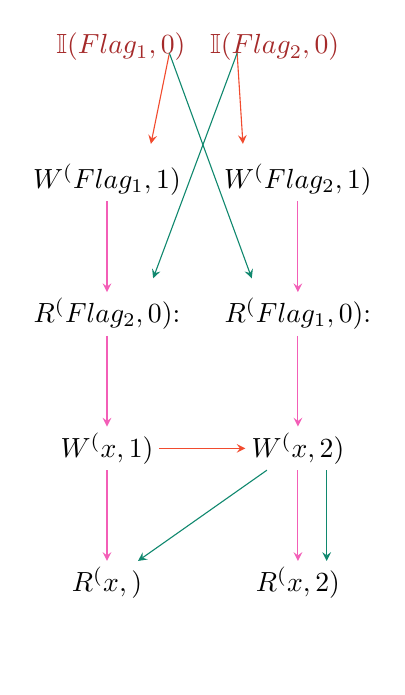
\begin{tikzpicture}[x=1em,y=1em,yscale=-1,xscale=-1]
	\tikzstyle{every node}=[font=\normalfont]
	
	\node (ifl1) [inner sep=2pt,color=Brown] {$\mathbb{I}(Flag_1,0)$};
	\node (ifl2) [right=30pt,inner sep=2pt,color=Brown] {$\mathbb{I}(Flag_2,0)$};
	
	\node (f11) [below left=10pt and -30pt of ifl1,inner sep=2pt, color=White] {$\mathbb{F}_{11}$};
	\node (fl1) [below=10pt of f11, inner sep=2pt] {$ W^\rlx(Flag_1,1) $};
	\node (f12) [below=10pt of fl1, inner sep=2pt, color=White] {$\mathbb{F}_{12}$};
	\node (rfl2) [below=10pt of f12, inner sep=2pt] {$R^\rlx(Flag_2,0)$:};
	\node (f13) [below=10pt of rfl2, inner sep=2pt, color=White] {$\mathbb{F}_{13}$};
	\node (cs11) [below=10pt of f13, inner sep=2pt] {$ W^\rlx(x,1) $};
	\node (f14) [below=10pt of cs11, inner sep=2pt, color=White] {$\mathbb{F}_{14}$};
	\node (cs12) [below=10pt of f14, inner sep=2pt] {$ R^\rlx(x,) $};
	\node (f15) [below=10pt of cs12, inner sep=2pt, color=White] {$\mathbb{F}_{15}$};
	
	\node (f21) [right=50pt of f11, inner sep=2pt, color=White] {$\mathbb{F}_{21}$};
	\node (fl2) [below=10pt of f21, inner sep=2pt] {$W^\rlx(Flag_2,1)$};
	\node (f22) [below=10pt of fl2, inner sep=2pt, color=White] {$\mathbb{F}_{22}$};
	\node (rfl1) [below=10pt of f22, inner sep=2pt] {$R^\rlx(Flag_1,0)$:};
	\node (f23) [below=10pt of rfl1, inner sep=2pt, color=White] {$\mathbb{F}_{23}$};
	\node (cs21) [below=10pt of f23, inner sep=2pt] {$ W^\rlx(x,2) $};
	\node (f24) [below=10pt of cs21, inner sep=2pt, color=White] {$\mathbb{F}_{24}$};
	\node (cs22) [below=10pt of f24, inner sep=2pt] {$ R^\rlx(x,2) $};
	\node (f25) [below=10pt of cs22, inner sep=2pt, color=White] {$\mathbb{F}_{23}$};
	%
	\draw [->,>=stealth,color=RedOrange] ($ (ifl1.south east)+(0.8,-5pt) $) -- node[pos=0.3,left=-2pt,font=\scriptsize,color=black] { $\lmo$ } ($ (fl1.north east)+(1.3,-5pt) $);
	\draw [->,>=stealth,color=RedOrange] ($ (ifl2.south west)+(-1.2,-5pt) $) -- node[pos=0.3,right=-2pt,font=\scriptsize,color=black] { $\lmo$ } ($ (fl2.north west)+(-0.9,-5pt) $);
	
	\draw [->,>=stealth,color=PineGreen] ($ (ifl1.south east)+(0.8,-5pt) $) -- node[pos=0.8,right=-2pt,font=\scriptsize,color=black] { $\lrf$ } ($ (rfl1.north west)+(-1.2,-5pt) $);
	\draw [->,>=stealth,color=PineGreen] ($ (ifl2.south west)+(-1.2,-5pt) $) -- node[pos=0.8,left=-2pt,font=\scriptsize,color=black] { $\lrf$ } ($ (rfl2.north east)+(1.2,-5pt) $);
	
	\draw [->,>=stealth,color=RedOrange] (cs11)  -- node[midway,above=-2pt,font=\scriptsize,color=black] { $\lmo$ } (cs21);
	\draw [->,>=stealth,color=PineGreen] (cs21)  -- node[midway,above=-2pt,font=\scriptsize,color=black] { $\lrf$ } (cs12);
	\draw [->,>=stealth,color=PineGreen] ($ (cs21.south)+(-10.4pt,0) $)  -- node[midway,right=-2pt,font=\scriptsize,color=black] { $\lrf$ } ($ (cs22.north)+(-10.4pt,0) $);
	
	\draw [->,>=stealth,color=CarnationPink] (fl1)  -- node[midway,right=-2pt,font=\scriptsize,color=black] { $\lsb$ } (rfl2);
	\draw [->,>=stealth,color=CarnationPink] (rfl2) -- node[midway,right=-2pt,font=\scriptsize,color=black] { $\lsb$ } (cs11);
	\draw [->,>=stealth,color=CarnationPink] (cs11) -- node[midway,right=-2pt,font=\scriptsize,color=black] { $\lsb$ } (cs12);
	
	\draw [->,>=stealth,color=CarnationPink] (fl2)  -- node[midway,right=-2pt,font=\scriptsize,color=black] { $\lsb$ } (rfl1);
	\draw [->,>=stealth,color=CarnationPink] (rfl1) -- node[midway,right=-2pt,font=\scriptsize,color=black] { $\lsb$ } (cs21);
	\draw [->,>=stealth,color=CarnationPink] (cs21) -- node[midway,right=-2pt,font=\scriptsize,color=black] { $\lsb$ } (cs22);
	
\end{tikzpicture}
} &
		\resizebox{0.24\textwidth}{!}{\tikzset{every picture/.style={line width=0.75pt}} %set default line width to 0.75pt        
\begin{tikzpicture}[x=1em,y=1em,yscale=-1,xscale=-1]
	\tikzstyle{every node}=[font=\normalfont]
	
	\node (ifl1) [inner sep=2pt,color=Brown] {$\mathbb{I}(Flag_1,0)$};
	\node (ifl2) [right=30pt,inner sep=2pt,color=Brown] {$\mathbb{I}(Flag_2,0)$};
	
	\node (f11) [below left=10pt and -30pt of ifl1,inner sep=2pt] {$\mathbb{F}_{11}$};
	\node (fl1) [below=10pt of f11, inner sep=2pt] {$ W^\sc(Flag_1,1) $};
	\node (f12) [below=10pt of fl1, inner sep=2pt] {$\mathbb{F}_{12}$};
	\node (rfl2) [below=10pt of f12, inner sep=2pt] {$R^\rlx(Flag_2,0)$:};
	\node (f13) [below=10pt of rfl2, inner sep=2pt] {$\mathbb{F}_{13}$};
	\node (cs11) [below=10pt of f13, inner sep=2pt] {$ W^\rlx(x,1) $};
	\node (f14) [below=10pt of cs11, inner sep=2pt] {$\mathbb{F}_{14}$};
	\node (cs12) [below=10pt of f14, inner sep=2pt] {$ R^\rlx(x,1) $};
	\node (f15) [below=10pt of cs12, inner sep=2pt] {$\mathbb{F}_{15}$};
	
	\node (f21) [right=50pt of f11, inner sep=2pt] {$\mathbb{F}_{21}$};
	\node (fl2) [below=10pt of f21, inner sep=2pt] {$W^\sc(Flag_2,1)$};
	\node (f22) [below=10pt of fl2, inner sep=2pt] {$\mathbb{F}_{22}$};
	\node (rfl1) [below=10pt of f22, inner sep=2pt] {$R^\rlx(Flag_1,0)$:};
	\node (f23) [below=10pt of rfl1, inner sep=2pt] {$\mathbb{F}_{23}$};
	\node (cs21) [below=10pt of f23, inner sep=2pt] {$ W^\rlx(x,2) $};
	\node (f24) [below=10pt of cs21, inner sep=2pt] {$\mathbb{F}_{24}$};
	\node (cs22) [below=10pt of f24, inner sep=2pt] {$ R^\rlx(x,1) $};
	\node (f25) [below=10pt of cs22, inner sep=2pt] {$\mathbb{F}_{23}$};
	%
	\draw [->,>=stealth,color=RedOrange] ($ (ifl1.south east)+(0.8,-5pt) $) -- node[pos=0.3,left=-2pt,font=\scriptsize,color=black] { $\lmo$ } ($ (fl1.north east)+(1.2,-5pt) $);
	\draw [->,>=stealth,color=RedOrange] ($ (ifl2.south west)+(-1.2,-5pt) $) -- node[pos=0.3,right=-2pt,font=\scriptsize,color=black] { $\lmo$ } ($ (fl2.north west)+(-0.7,-5pt) $);
	
	\draw [->,>=stealth,color=PineGreen] ($ (ifl1.south east)+(0.8,-5pt) $) -- node[pos=0.8,right=-2pt,font=\scriptsize,color=black] { $\lrf$ } ($ (rfl1.north west)+(-1.2,-5pt) $);
	\draw [->,>=stealth,color=PineGreen] ($ (ifl2.south west)+(-1.2,-5pt) $) -- node[pos=0.8,left=-2pt,font=\scriptsize,color=black] { $\lrf$ } ($ (rfl2.north east)+(1.2,-5pt) $);
	
	\draw [->,>=stealth,color=RedOrange] (cs11)  -- node[midway,above=-2pt,font=\scriptsize,color=black] { $\lmo$ } (cs21);
	\draw [->,>=stealth,color=PineGreen] (cs21)  -- node[midway,above=-2pt,font=\scriptsize,color=black] { $\lrf$ } (cs12);
	\draw [->,>=stealth,color=PineGreen] ($ (cs21.south)+(-10.4pt,0) $)  -- node[midway,right=-2pt,font=\scriptsize,color=black] { $\lrf$ } ($ (cs22.north)+(-10.4pt,0) $);
	
	\draw [->,>=stealth,color=CarnationPink] (f11)  -- node[midway,right=-2pt,font=\scriptsize,color=black] { $\lsb$ } (fl1);
	\draw [->,>=stealth,color=CarnationPink] (fl1)  -- node[midway,right=-2pt,font=\scriptsize,color=black] { $\lsb$ } (f12);
	\draw [->,>=stealth,color=CarnationPink] (f12)  -- node[midway,right=-2pt,font=\scriptsize,color=black] { $\lsb$ } (rfl2);
	\draw [->,>=stealth,color=CarnationPink] (rfl2) -- node[midway,right=-2pt,font=\scriptsize,color=black] { $\lsb$ } (f13);
	\draw [->,>=stealth,color=CarnationPink] (f13)  -- node[midway,right=-2pt,font=\scriptsize,color=black] { $\lsb$ } (cs11);
	\draw [->,>=stealth,color=CarnationPink] (cs11) -- node[midway,right=-2pt,font=\scriptsize,color=black] { $\lsb$ } (f14);
	\draw [->,>=stealth,color=CarnationPink] (f14)  -- node[midway,right=-2pt,font=\scriptsize,color=black] { $\lsb$ } (cs12);
	\draw [->,>=stealth,color=CarnationPink] (cs12) -- node[midway,right=-2pt,font=\scriptsize,color=black] { $\lsb$ } (f15);
	
	\draw [->,>=stealth,color=CarnationPink] (f21)  -- node[midway,right=-2pt,font=\scriptsize,color=black] { $\lsb$ } (fl2);
	\draw [->,>=stealth,color=CarnationPink] (fl2)  -- node[midway,right=-2pt,font=\scriptsize,color=black] { $\lsb$ } (f22);
	\draw [->,>=stealth,color=CarnationPink] (f22)  -- node[midway,right=-2pt,font=\scriptsize,color=black] { $\lsb$ } (rfl1);
	\draw [->,>=stealth,color=CarnationPink] (rfl1) -- node[midway,right=-2pt,font=\scriptsize,color=black] { $\lsb$ } (f23);
	\draw [->,>=stealth,color=CarnationPink] (f23)  -- node[midway,right=-2pt,font=\scriptsize,color=black] { $\lsb$ } (cs21);
	\draw [->,>=stealth,color=CarnationPink] (cs21) -- node[midway,right=-2pt,font=\scriptsize,color=black] { $\lsb$ } (f24);
	\draw [->,>=stealth,color=CarnationPink] (f24)  -- node[midway,right=-2pt,font=\scriptsize,color=black] { $\lsb$ } (cs22);
	\draw [->,>=stealth,color=CarnationPink] (cs22) -- node[midway,right=-2pt,font=\scriptsize,color=black] { $\lsb$ } (f25);
	
\end{tikzpicture}
} \\
		\hline
		
		\multicolumn{1}{c}{\hl{mutex-bt1}} &
		\multicolumn{1}{c}{$\imm{\hl{mutex-bt1}}$}  &
		\multicolumn{1}{c}{\hl{mutex-bt2}} &
		\multicolumn{1}{c}{$\imm{\hl{mutex-bt2}}$} \\
		
		\multicolumn{1}{c}{buggy trace 1} &
		\multicolumn{1}{c}{intermediate} &
		\multicolumn{1}{c}{buggy trace 2} &
		\multicolumn{1}{c}{intermediate} \\
	
		\multicolumn{1}{c}{} &
		\multicolumn{1}{c}{buggy trace 1} &
		\multicolumn{1}{c}{} &
		\multicolumn{1}{c}{buggy trace 2} \\
	\end{tabular}
\end{figure}

Algorithm~\ref{alg:main algo} iterates over each buggy trace
$\tau$ (line 4) and transforms the trace to an intermediate 
trace $\imm{\tau}$ (line 5). The algorithm further updates the 
event relations accordingly (line 6). As discussed in Section
\ref{sec:invalidating ce} a change is witnessed in the 
$\setHB$ relation. The transformed intermediate traces 
corresponding to buggy traces \hlref{mutex-bt1} and 
\hlref{mutex-bt2}, along with the updated event relations are 
represented in $\imm{\hlref{mutex-bt1}}$ and 
$\imm{\hlref{mutex-bt2}}$ respectively.

\noindent
{\bf Detecting cyclic relations indicating violation of 
	trace coherence}
In each intermediate buggy trace, the algorithm proceeds 
to perform \wkfence (line 7) and return cycles in compositions 
of event relations that define a coherence condition 
(Section~\ref{sec:c11}). For the intermediate traces 
$\imm{\hlref{mutex-bt1}}$ and $\imm{\hlref{mutex-bt2}}$
\wkfence would return an empty set.
%
The algorithm then proceeds to perform \stfence (line 8) that 
computes the $\so{\imm{\tau}}{}{}$ relation on \sc 
events and returns the cycles in $\so{\imm{\tau}}{}{}$.
The cyclic $\so{\imm{\tau}}{}{}$ relations in the intermediate
traces $\imm{\hlref{mutex-bt1}}$ and $\imm{\hlref{mutex-bt2}}$
are shown in $\imm{\hlref{mutex-bt1-so}}$ and 
$\imm{\hlref{mutex-bt2-so}}$. Note that, $\so{\imm{\tau}}{}{}$ 
would also be formed between every fence before 
$\mathbb{F}^\sc_{13}$ and every fence including and after 
$\mathbb{F}^\sc_{24}$ in $\imm{\hlref{mutex-bt1-so}}$ 
(correspondingly in $\imm{\hlref{mutex-bt1-so}}$), however, we 
have skipped the edges in the figures for better readability.

\begin{figure}[!h]
	\begin{tabular}{|c|c|}
		\hline
		\resizebox{0.24\textwidth}{!}{\tikzset{every picture/.style={line width=0.75pt}} %set default line width to 0.75pt        
\begin{tikzpicture}[x=1em,y=1em,yscale=-1,xscale=-1]
	\tikzstyle{every node}=[font=\normalfont]
	
	\node (ifl1) [inner sep=2pt,color=Brown] {$\mathbb{I}(Flag_1,0)$};
	\node (ifl2) [right=30pt,inner sep=2pt,color=Brown] {$\mathbb{I}(Flag_2,0)$};
	
	\node (f11) [below left=10pt and -30pt of ifl1,inner sep=2pt] {$\mathbb{F}^\sc_{11}$};
	\node (fl1) [below=10pt of f11, inner sep=2pt] {$ W^\sc(Flag_1,1) $};
	\node (f12) [below=10pt of fl1, inner sep=2pt] {$\mathbb{F}^\sc_{12}$};
	\node (rfl2) [below=10pt of f12, inner sep=2pt] {$R^\rlx(Flag_2,0)$:};
	\node (f13) [below=10pt of rfl2, inner sep=2pt] {$\mathbb{F}^\sc_{13}$};
	\node (cs11) [below=10pt of f13, inner sep=2pt] {$ W^\rlx(x,1) $};
	\node (f14) [below=10pt of cs11, inner sep=2pt] {$\mathbb{F}^\sc_{14}$};
	\node (cs12) [below=10pt of f14, inner sep=2pt] {$ R^\rlx(x,1) $};
	\node (f15) [below=10pt of cs12, inner sep=2pt] {$\mathbb{F}^\sc_{15}$};
	
	\node (f21) [right=50pt of f11, inner sep=2pt] {$\mathbb{F}^\sc_{21}$};
	\node (fl2) [below=10pt of f21, inner sep=2pt] {$W^\sc(Flag_2,1)$};
	\node (f22) [below=10pt of fl2, inner sep=2pt] {$\mathbb{F}^\sc_{22}$};
	\node (rfl1) [below=10pt of f22, inner sep=2pt] {$R^\rlx(Flag_1,0)$:};
	\node (f23) [below=10pt of rfl1, inner sep=2pt] {$\mathbb{F}^\sc_{23}$};
	\node (cs21) [below=10pt of f23, inner sep=2pt] {$ W^\rlx(x,2) $};
	\node (f24) [below=10pt of cs21, inner sep=2pt] {$\mathbb{F}^\sc_{24}$};
	\node (cs22) [below=10pt of f24, inner sep=2pt] {$ R^\rlx(x,1) $};
	\node (f25) [below=10pt of cs22, inner sep=2pt] {$\mathbb{F}^\sc_{23}$};
	%
	
	\draw [->,>=stealth,color=Mahogany] (f11)  -- node[pos=0.2,right=-2pt,font=\scriptsize,color=black] { $\lso$ } (f12);
	\draw [->,>=stealth,color=Mahogany] (f12)  -- node[pos=0.2,right=-2pt,font=\scriptsize,color=black] { $\lso$ } (f13);
	\draw [->,>=stealth,color=Mahogany] (f13)  -- node[pos=0.2,right=-2pt,font=\scriptsize,color=black] { $\lso$ } (f14);
	\draw [->,>=stealth,color=Mahogany] (f14)  -- node[pos=0.2,right=-2pt,font=\scriptsize,color=black] { $\lso$ } (f15);
	
	\draw [->,>=stealth,color=Mahogany] (f21)  -- node[pos=0.2,right=-2pt,font=\scriptsize,color=black] { $\lso$ } (f22);
	\draw [->,>=stealth,color=Mahogany] (f22)  -- node[pos=0.2,right=-2pt,font=\scriptsize,color=black] { $\lso$ } (f23);
	\draw [->,>=stealth,color=Mahogany] (f23)  -- node[pos=0.2,right=-2pt,font=\scriptsize,color=black] { $\lso$ } (f24);
	\draw [->,>=stealth,color=Mahogany] (f24)  -- node[pos=0.2,right=-2pt,font=\scriptsize,color=black] { $\lso$ } (f25);
	
	\draw [->,>=stealth,color=Mahogany] ($ (f12.north east) $)  to[out=-165,in=-15] node[midway,above=-2pt,font=\scriptsize,color=black] { $\lso$ } ($ (f22.north west) $);
	\draw [->,>=stealth,color=Mahogany] ($(f22.south west)$)  to[out=15,in=165] node[midway,below=-2pt,font=\scriptsize,color=black] { $\lso$ } ($(f12.south east)$);
	
	\draw [->,>=stealth,color=Mahogany] (f13)  -- node[midway,above=-2pt,font=\scriptsize,color=black] { $\lso$ } (f24);
	\draw [->,>=stealth,color=Mahogany] ($(f13.south east)$)  to[out=155,in=0] node[midway,left=-2pt,font=\scriptsize,color=black] { $\lso$ } ($(f25.west)$);
	
\end{tikzpicture}
} &
		\resizebox{0.24\textwidth}{!}{\tikzset{every picture/.style={line width=0.75pt}} %set default line width to 0.75pt        
\begin{tikzpicture}[x=1em,y=1em,yscale=-1,xscale=-1]
	\tikzstyle{every node}=[font=\normalfont]
	
	\node (ifl1) [inner sep=2pt,color=Brown] {$\mathbb{I}(Flag_1,0)$};
	\node (ifl2) [right=30pt,inner sep=2pt,color=Brown] {$\mathbb{I}(Flag_2,0)$};
	
	\node (f11) [below left=10pt and -30pt of ifl1,inner sep=2pt] {$\mathbb{F}^\sc_{11}$};
	\node (fl1) [below=10pt of f11, inner sep=2pt] {$ W^\sc(Flag_1,1) $};
	\node (f12) [below=10pt of fl1, inner sep=2pt] {$\mathbb{F}^\sc_{12}$};
	\node (rfl2) [below=10pt of f12, inner sep=2pt] {$R^\rlx(Flag_2,0)$:};
	\node (f13) [below=10pt of rfl2, inner sep=2pt] {$\mathbb{F}^\sc_{13}$};
	\node (cs11) [below=10pt of f13, inner sep=2pt] {$ W^\rlx(x,1) $};
	\node (f14) [below=10pt of cs11, inner sep=2pt] {$\mathbb{F}^\sc_{14}$};
	\node (cs12) [below=10pt of f14, inner sep=2pt] {$ R^\rlx(x,1) $};
	\node (f15) [below=10pt of cs12, inner sep=2pt] {$\mathbb{F}^\sc_{15}$};
	
	\node (f21) [right=50pt of f11, inner sep=2pt] {$\mathbb{F}^\sc_{21}$};
	\node (fl2) [below=10pt of f21, inner sep=2pt] {$W^\sc(Flag_2,1)$};
	\node (f22) [below=10pt of fl2, inner sep=2pt] {$\mathbb{F}^\sc_{22}$};
	\node (rfl1) [below=10pt of f22, inner sep=2pt] {$R^\rlx(Flag_1,0)$:};
	\node (f23) [below=10pt of rfl1, inner sep=2pt] {$\mathbb{F}^\sc_{23}$};
	\node (cs21) [below=10pt of f23, inner sep=2pt] {$ W^\rlx(x,2) $};
	\node (f24) [below=10pt of cs21, inner sep=2pt] {$\mathbb{F}^\sc_{24}$};
	\node (cs22) [below=10pt of f24, inner sep=2pt] {$ R^\rlx(x,1) $};
	\node (f25) [below=10pt of cs22, inner sep=2pt] {$\mathbb{F}^\sc_{23}$};
	%
	
	\draw [->,>=stealth,color=Mahogany] (f11)  -- node[pos=0.2,right=-2pt,font=\scriptsize,color=black] { $\lso$ } (f12);
	\draw [->,>=stealth,color=Mahogany] (f12)  -- node[pos=0.2,right=-2pt,font=\scriptsize,color=black] { $\lso$ } (f13);
	\draw [->,>=stealth,color=Mahogany] (f13)  -- node[pos=0.2,right=-2pt,font=\scriptsize,color=black] { $\lso$ } (f14);
	\draw [->,>=stealth,color=Mahogany] (f14)  -- node[pos=0.2,right=-2pt,font=\scriptsize,color=black] { $\lso$ } (f15);
	
	\draw [->,>=stealth,color=Mahogany] (f21)  -- node[pos=0.2,right=-2pt,font=\scriptsize,color=black] { $\lso$ } (f22);
	\draw [->,>=stealth,color=Mahogany] (f22)  -- node[pos=0.2,right=-2pt,font=\scriptsize,color=black] { $\lso$ } (f23);
	\draw [->,>=stealth,color=Mahogany] (f23)  -- node[pos=0.2,right=-2pt,font=\scriptsize,color=black] { $\lso$ } (f24);
	\draw [->,>=stealth,color=Mahogany] (f24)  -- node[pos=0.2,right=-2pt,font=\scriptsize,color=black] { $\lso$ } (f25);
	
	\draw [->,>=stealth,color=Mahogany] ($ (f12.north east) $)  to[out=-165,in=-15] node[midway,above=-2pt,font=\scriptsize,color=black] { $\lso$ } ($ (f22.north west) $);
	\draw [->,>=stealth,color=Mahogany] ($(f22.south west)$)  to[out=15,in=165] node[midway,below=-2pt,font=\scriptsize,color=black] { $\lso$ } ($(f12.south east)$);
	
	\draw [->,>=stealth,color=Mahogany] (f23)  -- node[midway,above=-2pt,font=\scriptsize,color=black] { $\lso$ } (f14);
	\draw [->,>=stealth,color=Mahogany] ($(f23.south west)$)  to[out=25,in=180] node[midway,right=-2pt,font=\scriptsize,color=black] { $\lso$ } ($(f15.east)$);
	
\end{tikzpicture}
} \\
		\hline
		
		\multicolumn{1}{c}{$\imm{\hl{mutex-bt1-so}}$}  &
		\multicolumn{1}{c}{$\imm{\hl{mutex-bt2-so}}$-} \\
		
		\multicolumn{1}{c}{intermediate} &
		\multicolumn{1}{c}{intermediate} \\
		
		\multicolumn{1}{c}{buggy trace 1} &
		\multicolumn{1}{c}{buggy trace 2} \\
	\end{tabular}
\end{figure}


\subsection{Reducing Fence Synthesis to SAT problem}
Recall that transitive closure of $ \so{\imm{\tau}}{}{} $ is same as 
$ \to{\imm{\tau}}{}{} $ in a valid \cc trace. Since  
$ \to{\imm{\tau}}{}{} $ is a total order, a valid \cc trace should not 
have a cycle in $ \so{\imm{\tau}}{}{} $. Conversely, if a trace has 
$ \so{\imm{\tau}}{}{} $-cycle, it cannot be a valid \cc trace. 
In order to make a trace $ \tau $ invalid under \cc, we force a \lso-cycle by inserting appropriate fences. 
Since $ \imm{\tau} $ assumes \mosc fences at all possible program locations,
any such cycle must exists in $ \so{\imm{\tau}}{}{} $. 
Hence, our problem is reduced to finding appropriate cycle in 
$\so{\imm{\tau}}{}{} $ and introducing these fences in the program to 
invalidate the trace $ \tau $.
If we introduced enough fences to cause at least \lso-cycle in 
every counter example, we stop all the buggy trace. 
It is possible that a counter example $ \tau $ does not have any 
$\so{\imm{\tau}}{}{}$-cycles. Since $ \imm{\tau} $ has \mosc fences at all 
possible program locations, we cannot add fences in such a trace to 
make it invalid \cc trace. 
Line 8 in Algorithm~\ref{alg:fence-syn} computes set $\so{\imm{\tau}}{}{}$-cycles. 
The problem of finding cycles in a graph is well-studied area. Hence, we 
choose to skip the details of this step.
If there are no $\so{\imm{\tau}}{}{}$-cycle in some $ \tau $, we conclude 
that it is not possible to stop this trace using \cc fences in lines 
9-11.


Let $ \cycles{\imm{\tau}} $ be the set of \lso-cycles in a trace $ \imm{\tau} $, 
where a cycle $ c \in \cycles{\imm{\tau}} $ is ordered sequence of 
$ \ordevents{\sc} $. We abuse the notation $\ordevents{\sc}_c$ to 
represent the set of events in a cycle $ c $. 
All the read and write events in $\ordevents{\sc}_c$ are already in program $ P $. 
Hence, to introduce a cycle $ c $ in the trace, we add the fences in $\ordevents{\sc}_c$, i.e, 
$\ordfences{\sc}_c$, in the program $ P $.
In other words, a cycle $ c $ can be introduced in a program if we insert 
$ (\bigwedge\limits_{f \in \ordfences{\sc}_c} f)$ fences in the program $ P $, 
where the truth assignment to a fence corresponds to inserting that fence 
in the program.
Recall that we need to stop at least one cycle from the set 
$ \cycles{\imm{\tau}} $ in order to make a trace $ \tau $ invalid.
Hence we need to insert $ (\bigvee\limits_{c \in \cycles{\imm{\tau}}} (\bigwedge\limits_{\fn{} \in \ordevents{\sc}_c \intersection 
\ordfences{\sc}} \fn{})) $ to stop a trace $ \tau $. 
We use $\formula{\so{\imm{\tau}}{}{}}$ to represent the boolean formula 
corresponding to the $ \so{\imm{\tau}}{}{} $-cycles.
Clearly, any satisfying assignment to $ \formula{\so{\imm{\tau}}{}{}} $ 
will give list of fences required to stop the buggy trace $ \tau $.
%
Furthermore, we construct the formula for all trace 
$ \tau \in \mathcal{CE} $ by conjuncting them in 
line 12 of Algorithm~\ref{alg:fence-syn}, i.e., 
at the end of the for loop in lines 4-12, the formula 
$ \phi \definedas (\bigwedge\limits_{\tau \in \mathcal{CE}} 
(\bigvee\limits_{c \in \cycles{\imm{\tau}}} 
(\bigwedge\limits_{\fn{} \in \ordevents{\sc}_c \intersection \ordfences{\sc}} \fn{}))) $.
Any satisfying assignment of the formula $\phi$ will list the fences that 
are enough to stop the buggy traces in $ \mathcal{CE} $.

%\begin{lemma}
%	Introducing fences in any $\so{\imm{\tau}}{}{}$-cycle will stop the counter example $ \tau $ in actual trace of the program.
%\end{lemma}

\begin{lemma}
	If there are no cycles in $\so{\imm{\tau}}{}{}$ of a buggy trace 
	$\tau$, the counter-example $ \tau $ cannot be stopped using any \cc 
	fences.
\end{lemma}

\begin{theorem}
	Any satisfying assignment to $ \formula{\so{\imm{\tau}}{}{}} $ 
	will give list of fences required to stop the buggy trace $ \tau $
\end{theorem}


\subsection{Finding Optimal Placement of the Fences}
One possible satisfying assignment to formula $ \phi $ is assigning the 
value true to all fences. Clearly such a solution is very expensive.
The number of truth assignments in the solution of formula $ \phi $ is 
equal to the number of fences inserted in the program.
%A satisfying assignment of the formula $ \phi $ with lesser number 
%of fences will give us a more optimal fence placement. 
Hence, a satisfying assignment of the formula $ \phi $ with the least 
number of fences will give us the optimal fence placement. 
Therefore, we reduce the problem of finding optimal fence placement to the 
minimal model of a SAT formula. 

The problem of minimal model computation has been studied in 
\divComment{need references}. \divComment{Need complexity argument for min model}.

In some cases, a fence at certain program location maybe more expensive 
than at other program location. For example, a fence inside a loop is may 
execute several times. Hence, such a fence may be more expensive than a 
fence placed outside the loop body.
%
\ourtechnique can handle such constraints by using weighted minimal model 
problem \divComment{need references}, where weight of each fence 
corresponds how expensive the fence is. 
The Algorithm~\ref{alg:fence-syn} can be modified to take weight 
function as input. 
%
The current implementation of \ourtechnique uses repeated calls to Z3 SAT 
solver to find the minimal model. \divComment{How are we solving it?}


\begin{theorem}
	For any input program $ P $, minimal model of $ \phi $ gives optimal
	number of fences required to stop all the buggy traces in 
	$ \mathcal{CE} $.
\end{theorem}



\section{Implementation/Tool Description}
\par
The tool is written using the python programming language. 
It takes the location of the input program using the \textit{-f} 
flag. The first step is to obtain a list of buggy executions 
from any C11 verification tool. 
The output from verification tool is obtained 
in the form of a list of buggy executions which is then formatted 
and translated into data structures for our usage. Each of these 
buggy executions are run through a series of steps as described in 
\textsection \ref{sec:methodology} - finding \lhb, \lmo, adding pseudo fences. 
finding \lto, finding cycles, eliminating fences and inserting them 
back into the program.

The tool makes use of the following python packages and libraries:
\divComment{add reference}
\begin{itemize}
	\item networkx - for graphing related queries - finding cycles
	\item operator
	\item shlex
	\item argparse
	\item os
\end{itemize}

The following python functions and other optimizations have
been applied for faster processing:
\begin{itemize}
	\item lambda function to sort traces according to thread number faster
	\item \texttt{enumerate} function to make list search faster
	\item \texttt{index} function to index quicker
	\item values converted to int at the beginning while translating model checker output for faster lookup
	\item no need to compute transitive \sc edges
	\item use \texttt{networkx} library that uses Johnson's 
	algorithm to enumerate all the cycles in a graph
	\item using memoization to store instruction metadata
\end{itemize}


\subsection{Finding and Pre-processing Buggy Executions}
The tool begins by translating model checker output obtained from a 
terminal subprocess, spawned from the main process running the tool. 
Subsequently, one may choose to use any model checker by creating a 
custom translator for it. Any translator would need to run the input program in the model checker, 
obtain the output containing a list of buggy executions and 
extract the following important information from each instruction 
of each trace:
%
\begin{enumerate}
	\item thread number of the instruction
	\item instruction type (thread create/ thread start/ init/ atomic read/ atomic write/ atomic rmw)
	\item memory order (relaxed, acquire, release, acq\textunderscore rel, seq\textunderscore cst)
	\item memory address (variable name in the system)
	\item rf value (in case of read/rmw instruction)
	\item line number for each instruction
\end{enumerate}
For any of the above meta-data, if a field does not apply for a certain instruction, 
it is given the value ``NA''. In case any information is missing from 
the model checker outputs, the model checker should be revised in order 
to obtain and print that piece of information. 
%
Since we are providing a prototype tool, 
currently, we provide translator only for CDSChecker. 
We choose to use CDSChecker for the following reasons- 
\begin{itemize}
	\item CDSChecker is an open source tool. Hence we were able 
	to modify the source code to suite our needs (explained below).
	
	\item Most other tools in domain provide results only in binary formats.
	CDSChecker gives a detailed output of all the required information.
	
	\item Most of the alternative tools do not focus C11 in its entirety, 
	but a subset of similar memory model.
	
	\item The output of CDSChecker provides more information 
	(such as the value read/written) than other tools in the domain.
\end{itemize}
Existing model checkers such as \textsc{RCMC}\cite{rcmc-POPL18},  
\textsc{GenMC}\cite{genmc-OOPSLA19,genmc-PLDI19} are based on and created for the 
repaired sequential consistency model RC11\cite{LahavVafeiadis-PLDI17}.
\textsc{Tracer}\cite{tracer2018} is only for RA fragment of C11.
Whereas a tool such as Herd\cite{herd} is not a 
robust enough tool which can be used for our purposes. 
\ishComment{nidhugg does not suppport C11}

The input file is first copied to the CDSChecker test folder and 
verified using CDSChecker. 
For our purposes, we have re-written some of the code in CDSChecker 
so that it also and prints the line numbers of relevant instructions 
from the source code. We require the line number in order to know 
where to position the fences. We have also added flag \texttt{-c} 
in CDSChecker to specify number of buggy executions to output. In 
case flag \texttt{-c n} is provided the, CDSChecker stops the execution 
as soon as it finds \texttt{n} buggy executions.


\subsubsection{Extracting line numbers and tool requirements}
Line numbers are extracted in CDSChecker by adding an extra parameter 
to the atomic functions. This extra parameter takes an integer input. 
Wecreated wrapped functions of atomic load, store and rmw functions 
to take this extra parameter, which is then passed and printed in 
output traces. As a result, in the input program each of these 
instructions is also modified and the first parameter is always 
given as {\tt{\textunderscore\textunderscore LINE\textunderscore\textunderscore}}.

We expect input program to abide by the following rules:
\begin{enumerate}
	\item atomic load, store, rmw functions need to have 
	``{\tt{\textunderscore\textunderscore LINE\textunderscore\textunderscore}}'' 
	as the first parameter.
	\item if statements and loops need to be scoped with 
	brackets % always(in case fences are inserted inside them)
	\item only sc fences are allowed if the input program 
	already contains fences
	\item no two consecutive instructions in a program should be fences 
	\item filename cannot end with ``\_fence''
	\item if there are other functions apart from thread functions 
	containing atomic operations, they need to be unrolled inside the 
	thread functions calling them because a fence maybe required only 
	in some calls to such functions.
\end{enumerate}

\textit{Note:} we have not changed the methodology of any of the functions
from CDSChecker. We have only added an extra functionality which is independant
and inobtrusive to the rest of the tool.

\subsubsection{Fence locations in Actual Program}\

Because of re-ordering and branching, the fence names might 
differ for each trace while mapping back to the source program. 
For example, in some program $F_1n_5$ may come after line 12 
for one trace and line 15 for another trace. For the purpose of this 
example, let us assume each fence to be a position in the original 
source code instead of it being a fence position in a single trace. 
This way, fence $F_4$ is the same fence for both the traces 
with respect to its position in the source code, which can be found 
out using line numbers.

\subsection{Data structures used}
\lhb relation, since there are many, are stored as boolean values in 
an adjacency table, as opposed to the ``list of tuples'' format used for 
all other relations in the tool. The adjacency table is indexed based 
on the instruction number as given by CDSChecker. 
%An example can be 
%seen in Fig \ref{fig:cds_hb}. The 0 index is left out as empty and 
%filled with 0's, while a 1 for row 3 column 4 would mean \hb{3}{4}.

\begin{itemize}
	\item adjacency matrix to store \lhb relations because the size 
	of \lhb is usually large
	\item list of tuples to store relations \lmo, \lsb, \sc
	since the size of these relations is small and finding cycle is
	easier
	\item list of lists to store traces and instruction information
\end{itemize}

\subsection{A time saving optimization} \label{sec:opti}
For input programs with an enormous number of possibilities, the 
tool might take some time to complete the analysis for each and 
every trace. Providing an alternative for this, we have also 
introduced an optional flag \texttt{-t} to specify the number 
of traces to analyze at a time until the solution is found. 
If the value is specified as \texttt{-t 3}, the tool will look 
at only the first 3 buggy executions from the model checker and 
base the analysis on them. It will then add fences in the input 
program according to the first 3 traces and then analyze this 
new program again. It will keep running the program after 
adding fences until a conclusion is reached. This would save 
time on the user's part but it may compromise on the optimality, 
since there might be more fences added with this method as compared 
with the original method. There is also an additional optional 
flag \texttt{-m} to specify the maximum number of iterations to 
be run. On specifying this value, the analysis will stop at the 
\textit{m}th iteration if the program is buggy at that point.



\section{Results}

\section{Conclusion and future work}

\bibliographystyle{unsrtnat}
\bibliography{References.bib}
\end{document}
